\documentclass[a4paper,11pt]{article}

\usepackage[utf8]{inputenc}
\usepackage{microtype}
\usepackage[DIV=15]{typearea}
% \usepackage{geometry}
% \geometry{
% 	margin = 20mm
% }

%\usepackage{titlesec}
%\titleformat{\section}[block]{\sffamily\Large\filcenter\bfseries}{\S\thesection.}{0.25cm}{\Large}
%\titleformat{\subsection}[block]{\vspace{-0.7em}\large\bfseries\sffamily}{\S\S\thesubsection.}{0.2cm}{\large}
\usepackage[parfill]{parskip}
\setlength{\parindent}{0em}
\usepackage{enumitem}
\usepackage{tocloft}
\usepackage[backend=biber,sorting=ynt]{biblatex}

\usepackage{amsmath, amssymb, amsfonts, amsthm, mathtools}
\usepackage{nccmath}
\newtheorem*{note}{Note}
\newtheorem*{hint}{Hint}
\theoremstyle{remark}
\newtheorem*{sol}{Solution}
\usepackage{algorithm}
\usepackage{algpseudocode}
% \usepackage[linesnumbered,ruled]{algorithm2e}

\usepackage{tikz}
\usetikzlibrary{shapes,arrows.meta}
\tikzstyle{line} = [draw, -{Latex[length=1mm,width=2mm]}]
\tikzstyle{linedash} = [draw, dash dot]

% \usepackage{pdfpages}
%t\usetikzlibrary{quotes}
\usepackage{graphicx}
\graphicspath{{./Images}}
\usepackage{booktabs,array}
\usepackage{subcaption}
\usepackage{wrapfig}
\usepackage{float}
% \usepackage{minted}

\usepackage{datetime2}
\usepackage{relsize}
\usepackage{url}
\usepackage{cprotect}
\usepackage{comment}
\usepackage{lipsum}
\usepackage{epigraph}

\usepackage{multirow}
\usepackage{xhfill}
\usepackage{xcolor}

\usepackage{fancyhdr}
%\pagestyle{fancy}
%\lhead{\textsc{Game Theory}}
%\rhead{\textsc{Param Rathour}}
\usepackage[colorlinks=true]{hyperref}
\hypersetup{
	linktoc= all,     %set to all if you want both sections and subsections linked
	urlcolor=magenta,
	pdftitle={Computational Commutative Algebra and Geometry},
	pdfauthor = {Param Rathour, Department of Electrical Engineering, Indian Institute of Technology Bombay},
	    pdfsubject={EE451 Supervised Research Exposition, Prof. Debasattam Pal}
}
%\renewcommand\familydefault{\sfdefault}
\renewcommand{\d}{\, \mathrm{d}}
\newcommand{\I}{\textbf{I}}
\newcommand{\V}{\textbf{V}}
\newcommand{\F}{\ensuremath\mathbb{F}}
\newcommand{\R}{\ensuremath\mathbb{R}}
\newcommand{\C}{\ensuremath\mathbb{C}}
\newcommand{\Q}{\ensuremath\mathbb{Q}}
\newcommand{\Z}{\ensuremath\mathbb{Z}}
\newcommand{\Zp}{\ensuremath\mathbb{Z}^+}
\newcommand{\lex}{\ensuremath>_{\text{lex}}}
\newcommand{\grlex}{\ensuremath>_{\text{grlex}}}
\newcommand{\grevlex}{\ensuremath>_{\text{grevlex}}}
\newcommand{\op}[1]{\operatorname{#1}}
\newcommand{\ditto}[1][.4pt]{\xrfill{#1}~\textquotedbl~\xrfill{#1}}
\newcommand{\suth}{\textsuperscript{th}}
\newcommand{\Grob}{Gr\"{o}bner }
\newcommand{\GrobB}{Gr\"{o}bner Bases}
\newcommand{\GrobBi}{Gr\"{o}bner Basis}
\renewcommand{\algorithmicrequire}{\textbf{Input:}}
\renewcommand{\algorithmicensure}{\textbf{Output:}}

% \renewcommand*{\thefootnote}{\fnsymbol{footnote}}
\addtocontents{toc}{\protect\setcounter{tocdepth}{1}}
\newcommand\at[2]{\left.#1\right|_{#2}}
\renewcommand\qedsymbol{$\blacksquare$}
\newcommand{\tani}{\tan^{-1}}
\newcommand{\sini}{\sin^{-1}}
\newcommand{\cosi}{\cos^{-1}}
\newcommand{\vLine}{\unskip\ \vrule\ }
\renewcommand{\arraystretch}{1.3}

%---------------------- ToC Lines ---------------------------%
\makeatletter
\renewcommand*\l@section{\@dottedtocline{1}{1.5em}{2.3em}}
\makeatother

%---------------------- Environments ---------------------------%
\makeatletter
\def\th@plain{%
  \thm@notefont{}% same as heading font
  \itshape % body font
}
\def\th@definition{%
  \thm@notefont{\textbf}% same as heading font
  \normalfont % body font
}
\makeatother

\numberwithin{equation}{section}
\numberwithin{figure}{section}
\numberwithin{table}{section}

\theoremstyle{definition}
\newtheorem{defn}{Definition}[section]
\newtheorem{theorem}[defn]{Theorem}
\newtheorem{lem}[defn]{Lemma}
\newtheorem{cor}[defn]{Corollary}
\newtheorem{prop}[defn]{Proposition}
\newtheorem{exm}[defn]{Example}

\newtheorem{ax}{Axiom}[section]

\theoremstyle{remark}
\newtheorem*{rem}{Remark}
\newtheorem*{Note}{Note}

%------------------------- Cover Page --------------------------------%
\renewcommand\epigraphflush{flushright}
\renewcommand\epigraphsize{\normalsize}
\renewcommand{\textflush}{flushepinormal}
\setlength\epigraphwidth{0.62\textwidth}

\definecolor{titlepagecolor}{cmyk}{1,.60,0,.40}

\DeclareFixedFont{\titlefont}{T1}{ppl}{b}{it}{2.5em}

\makeatletter                       
\def\printauthor{%                  
    {\large \@author}}              
\makeatother

% ------------------ Abstract and Acknoledgement --------------------- %
\usepackage{etoolbox}
\patchcmd{\abstract}{\titlepage}{}{}{}
\patchcmd{\endabstract}{\endtitlepage}{}{}{}

%---------------------- For Part 0 ------------------------------%
\makeatletter
\@addtoreset{section}{part}
\makeatother
\renewcommand\thepart{\Roman{part}}
% %----------------- For no vspace above proof ----------------- %
% \makeatletter
% \renewenvironment{proof}[1][\proofname]{\par
%   \vspace{-\topsep}% remove the space after the theorem
%   \pushQED{\qed}%
%   \normalfont
%   \topsep0pt \partopsep0pt % no space before
%   \trivlist
%   \item[\hskip\labelsep
%         \itshape
%     #1\@addpunct{.}]\ignorespaces
% }{%
%   \popQED\endtrivlist\@endpefalse
%   \addvspace{6pt plus 6pt} % some space after
% }
% \makeatother
\title{Computational Commutative Algebra and Geometry}
\author{%
    {\LARGE\textbf{Rathour Param Jitendrakumar}}\\[0.4em]
    {\Large 190070049}\\[0.4em]
    {\Large Department of Electrical Engineering}\\[0.4em]
    {\Large Indian Institue of Technology Bombay}\\[0.4em]
    %\texttt{paramrathour3435@gmail.com}\vspace{20pt}}\\
    {\Large  Guide: Prof. Debasattam Pal}}
\date{\today}
\addbibresource{references.bib}
%\includeonly{Files/Practice Problems 7}
%\includeonly{Files/Hints}

\begin{document}
\pagenumbering{gobble}
\begin{titlepage}
%\noindent
%\hfill
\vspace*{10em}
\begin{center}
  \titlefont Computational Commutative Algebra \newline\hspace*{2.5em} and Geometry
  \vspace*{1em}
  \newline \textsc{\LARGE Supervised Research Exposition}

\end{center}
\begin{comment}
\vspace*{4em}
\titlefont\ \ Game Theory\par
\epigraph{Mathematics, rightly viewed, possesses not only truth, but supreme beauty cold and austere, like that of sculpture, without appeal to any part of our weaker nature, without the gorgeous trappings of painting or music, yet sublimely pure, and capable of a stern perfection such as only the greatest art can show.
The true spirit of delight, the exaltation, the sense of being more than Man, which is the touchstone of the highest excellence, is to be found in mathematics as surely as in poetry.}%
{\textsc{Bertrand Russell}, \textit{Study of Mathematics}}
\null\vfill
\end{comment}
\vspace*{5em}
\begin{center}
  
\includegraphics[width=0.4\linewidth]{IIT_Bombay_Logo.pdf}
\end{center}
\vspace*{5em}
%\hfill
\begin{center}
\begin{minipage}{0.7\linewidth}
    \begin{center}
        \printauthor
    \end{center}
\end{minipage}
\end{center}
%
% \begin{minipage}{0.02\linewidth}
%     \rule{1pt}{125pt}
% \end{minipage}

% The following code is borrowed from: https://tex.stackexchange.com/a/86310/10898
\begin{tikzpicture}[remember picture,overlay,shorten >= -10pt]

\coordinate (aux1) at ([yshift=-15pt]current page.north east);
\coordinate (aux2) at ([yshift=-410pt]current page.north east);
\coordinate (aux3) at ([xshift=-4.5cm]current page.north east);
\coordinate (aux4) at ([yshift=-150pt]current page.north east);

\begin{scope}[titlepagecolor!40,line width=12pt,rounded corners=12pt]
\draw
  (aux1) -- coordinate (a)
  ++(225:5) --
  ++(-45:5.1) coordinate (b);
\draw[shorten <= -10pt]
  (aux3) --
  (a) --
  (aux1);
\draw[opacity=0.6,titlepagecolor,shorten <= -10pt]
  (b) --
  ++(225:2.2) --
  ++(-45:2.2);
\end{scope}
\draw[titlepagecolor,line width=8pt,rounded corners=8pt,shorten <= -10pt]
  (aux4) --
  ++(225:0.8) --
  ++(-45:0.8);
\begin{scope}[titlepagecolor!70,line width=6pt,rounded corners=8pt]
\draw[shorten <= -10pt]
  (aux2) --
  ++(225:3) coordinate[pos=0.45] (c) --
  ++(-45:3.1);
\draw
  (aux2) --
  (c) --
  ++(135:2.5) --
  ++(45:2.5) --
  ++(-45:2.5) coordinate[pos=0.3] (d);   
\draw 
  (d) -- +(45:1);
\end{scope}
\end{tikzpicture}%
\end{titlepage}
\begin{titlepage}
	\null\vspace{\fill}
	% \input{Files/Abstract}
	\begin{abstract}
		This report is divided into parts: An Introduction to Algebra and Geometry followed by An Introduction to \Grob Bases then Applications of \Grob Bases. 
		We start with an introduction to algebraic concepts, focussing over polynomials, ideals and their algorithms. Then we study geometric concepts such as varieties and their relationship with ideals which is probed with interesting problem. One such problem of ``Ideal Membership'' is broken down into simpler cases and the development of \Grob Bases Theory and Computation is motivated using it. Then, we focus on select applications of \Grob Bases from countless many available in literature and also discuss SageMath implementations for some of them.
		I have tried to make this report interesting and also covered fundamentals.
		Still, this is just a \emph{glimpse} of an extensive topic like \Grob Bases.
		Finally, I encourage you to look at all the SageMath programs and their diverse and exciting applications \href{https://github.com/paramrathour/Groebner-Basis-Applications}{here}.
	\end{abstract}
	\vspace{\fill}
	\renewcommand{\abstractname}{Acknowledgements}
	% \input{Files/Acknowledgements}
	\begin{abstract}
		This report was developed as a part of the course \emph{EE451: Supervised Research Exposition} to compile together my learnings and experiences.
		I thank my parents for always motivating me.
		I would also like to express gratitude to my guide: Prof. Debasattam for introducing me to this fascinating topic.
		Most of the content here is inspired by \cite{book:coxlittleoshea}, many statements are directly taken from here and my explanations are based on my understanding from the book.
		And, lastly thanks to you, reader, I have worked hard in making this report, in the hope that this work helps you in some way.
	\end{abstract}
	\vspace{\fill}
\end{titlepage}
\pagenumbering{roman}
\setcounter{tocdepth}{2}
\tableofcontents
\clearpage
\pagenumbering{arabic}
% \part{Introduction}
% Game theory is the study of mathematical models of strategic interaction among rational decision-makers.
Originally, it addressed zero-sum games, in which each participant's gains or losses are exactly balanced by those of the other participants.
In the 21st century, game theory applies to a wide range of behavioral relations, and is now an umbrella term for the science of logical decision making in humans, animals, and computers.
The term game used in the phrase game theory corresponds to an interaction involving decision makers or players who are rational and intelligent.
Informally, rationality of a player implies that the player chooses his strategies so as to maximize a well defined individualistic payoff while intelligence means that players are capable enough to compute their best strategies.

Traditional games such as chess and bridge represent games of a fairly straightforward nature.
Games that game theory deals with are much more general and could be viewed as abstractions and extensions of the traditional games.
The abstractions and extensions are powerful enough to include all complexities and characteristics of social interactions.
For this reason, game theory has proved to be an extremely valuable tool in social sciences in general and economics in particular.

While game theory is concerned with analysis of games, mechanism design is reverse engineering of games involving designing games with desirable outcomes.
% \subsection{Current Trends}
\section{Key Notions in Game Theory}
\subsection{Representation of Games}
There are two forms of representation. Namely,
\begin{itemize}
    \item Strategic Form (or Normal Form)
    \item Extensive Form
\end{itemize}
First we will look at Strategic Form Games also called as Normal Form Games, this is a very commonly used representation for games.
\subsubsection{Strategic Form}
A strategic form game is a simultaneous move game that captures each agent's decision problem of choosing a strategy that will counter the strategies adopted by the other agents.
Each player is faced with this problem and therefore the players can be thought of as simultaneously choosing their strategies from the respective sets $S_1,S_2,\ldots,S_n$.
A play of the game is as follows, each player simultaneously selects a strategy and informs this to a neutral observer who then computes the outcome and the utilities. Formally,
\begin{defn}[Strategic Form Game]{\label{def:sfg}}
    A Strategic Form Game $\Gamma$ is a tuple $\langle N,(S_i)_{i\in N},(u_i)_{i\in N}\rangle$, where
    \begin{itemize}
        \item $N=\{1,2,\ldots,n\}$ is a set of players
        \item $S_1,S_2,\ldots,S_n$ are sets called the strategy sets of the players $1,2,\ldots,n$ respectively
        \item $u_i : S_1 \times S_2 \times \cdots \times S_n \rightarrow \R$ for $i = 1, 2,\ldots, n$ are mappings called the utility functions or payoff functions.
    \end{itemize}
\end{defn}
The strategies are also called \textbf{actions} or more specifically \textbf{pure strategies}.
We denote the collection of all strategy profiles or strategy vectors of the players by the set $S$ which is the Cartesian product $S_1 \times S_2 \times \ldots \times S_n$.
\subsubsection{Extensive Form}
An Extensive Form of a game, is a representation of games in the form of a decision tree.
\begin{defn}[Extensive Form Game]{\label{def:efg}}
    An Extensive Form Game $\Gamma$ is a tuple 

    $\langle N,(A_i)_{i\in N},\mathbb{H},P,(\mathbb{I}_i)_{i\in N},(u_i)_{i\in N}\rangle$, where
    \begin{itemize}
        \item $N = {1, 2,\ldots,n}$ is a finite set of players
        \item $A_i$ for $i=1, 2,\ldots,n$ is the set of actions available to player $i$ (action set of player $i$)
        \item $\mathbb{H}$ is the set of all terminal histories where a terminal history is a path of actions from the root to a terminal node such that it is not a proper subhistory of any other terminal history. Denote by $S_\mathbb{H}$ the set of all proper subhistories (including the empty history $\varepsilon$) of all terminal histories.
        \item $P : S_\mathbb{H} \rightarrow N$ is a player function that associates each proper subhistory to a certain player
        \item $\mathbb{I}_i$ for $i = 1, 2,\ldots,n$ is the set of all information sets of player $i$
        \item $u_i : \mathbb{H} \rightarrow \R$ for $i = 1, 2,\ldots,n$ gives the utility of player $i$ corresponding to each terminal history.
    \end{itemize}
\end{defn}
\begin{exm}[Rock-Paper-Scissors]{\label{exm:rps}}
    This is an example of two player zero-sum game, where each player has three strategies, called rock, paper, and scissors.
    Two players simultaneously display one of three symbols: a rock, a paper, or scissors.
    The rock symbol beats scissors symbol; scissors symbol beats paper symbol; paper symbol beats rock symbol (symbolically, rock can break scissors; scissors can cut paper; and paper can cover rock).

    \textbf{Strategic Form:} The payoff matrix for this game is given as follows.
    \begin{table}[h]
        \centering
        \begin{tabular}{ |c|c|c|c| } 
            \hline
            1/2 & Rock & Paper & Scissors\\\hline
            Rock & $0,0$ & $-1,1$ & $1,-1$\\ \hline
            Paper & $1,-1$ & $0,0$ &$-1,1$\\ \hline
            Scissors & $-1,1$ & $1,-1$ & $0,0$\\\hline
        \end{tabular}
        \caption{Payoff Matrix for Rock Paper Scissors}
    \end{table}
    \begin{note}
    As a convention, Player 1 is called row player (as in this matrix, each row has same player 1's strategy) and Player 2 is called column player similarly
    \end{note}
    For this game,
    \begin{itemize}
    \item $N = \{1, 2\}$
    \item $S_1 = S_2 = \{\text{Rock}, \text{Paper}, \text{Scissors}\}$, let's denote it as \{R, P, S\}
    \item $u_1(R, R) = 0$, $u_1(R, P) = -1$, $u_1(R, S) = 1$, $u_1(P, R) = 1$, $u_1(P, P) = 0$, $u_1(P, S) = -1$, $u_1(S, R) = -1$, $u_1(S, P) = 1$, $u_1(S, S) = 0$
    \item $u_2(R, R) = 0$, $u_2(R, P) = 1$, $u_2(R, S) = -1$, $u_2(P, R) = -1$, $u_2(P, P) = 0$, $u_2(P, S) = 1$, $u_2(S, R) = 1$, $u_2(S, P) = -1$, $u_2(S, S) = 0$
    \end{itemize}
    \textbf{Extensive Form:}
    The extensive form for this game is given by the following game tree (A tree each with player 1 \& 2 as root node).
    \begin{figure}[H]
    \centering
    \begin{subfigure}{0.45\linewidth}
        \centering
        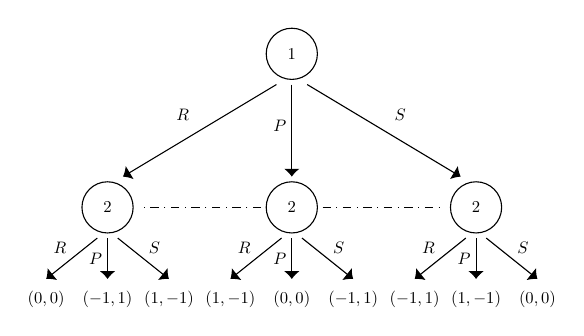
\begin{tikzpicture}[scale=0.13, every node/.style={scale=0.6}]
            \tikzstyle{every node}+=[inner sep=0pt]
                \draw [black] (36,-15) circle (2.5);
                \draw (36,-15) node {$1$};
                \draw [black] (36,-30) circle (2.5);
                \draw (36,-30) node {$2$};
                \draw [black] (54,-30) circle (2.5);
                \draw (54,-30) node {$2$};
                \draw [black] (18,-30) circle (2.5);
                \draw (18,-30) node {$2$};
                \draw (12,-39) node {$(0,0)$};
                \draw (18,-39) node {$(-1,1)$};
                \draw (24,-39) node {$(1,-1)$};
                \draw (30,-39) node {$(1,-1)$};
                \draw (36,-39) node {$(0,0)$};
                \draw (42,-39) node {$(-1,1)$};
                \draw (48,-39) node {$(-1,1)$};
                \draw (54,-39) node {$(1,-1)$};
                \draw (60,-39) node {$(0,0)$};
                \draw (26,-21) node [left] {$R$};
                \draw (36-0.5,-22) node [left] {$P$};
                \draw (46,-21) node [right] {$S$};
                \draw (14,-34) node [left] {$R$};
                \draw (18-0.5,-35) node [left] {$P$};
                \draw (22,-34) node [right] {$S$};
                \draw (32,-34) node [left] {$R$};
                \draw (36-0.5,-35) node [left] {$P$};
                \draw (40,-34) node [right] {$S$};
                \draw (50,-34) node [left] {$R$};
                \draw (54-0.5,-35) node [left] {$P$};
                \draw (58,-34) node [right] {$S$};
                \path [linedash] (39,-30) -- (51,-30);
                \path [linedash] (33,-30) -- (21,-30);
                \path [line] (36,-18) -- (36,-27);
                \path [line] (37.5,-18) -- (52.5,-27);
                \path [line] (34.5,-18) -- (19.5,-27);
                \path [line] (17,-33) -- (12,-37);
                \path [line] (18,-33) -- (18,-37);
                \path [line] (19,-33) -- (24,-37);
                \path [line] (35,-33) -- (30,-37);
                \path [line] (36,-33) -- (36,-37);
                \path [line] (37,-33) -- (42,-37);
                \path [line] (53,-33) -- (48,-37);
                \path [line] (54,-33) -- (54,-37);
                \path [line] (55,-33) -- (60,-37);
            \end{tikzpicture}
            \caption{Player 1 as root node}
            \label{fig:rps1}
    \end{subfigure}
    \vLine
    \begin{subfigure}{0.45\linewidth}
        \centering
        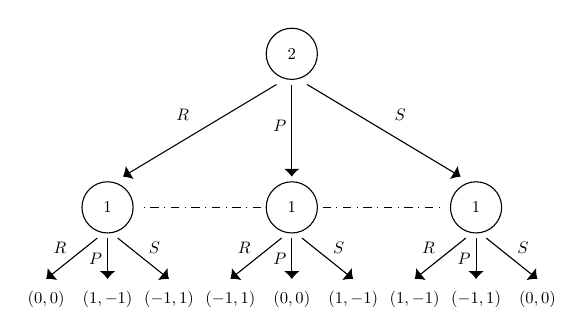
\begin{tikzpicture}[scale=0.13, every node/.style={scale=0.6}]
            \tikzstyle{every node}+=[inner sep=0pt]
                \draw [black] (36,-15) circle (2.5);
                \draw (36,-15) node {$2$};
                \draw [black] (36,-30) circle (2.5);
                \draw (36,-30) node {$1$};
                \draw [black] (54,-30) circle (2.5);
                \draw (54,-30) node {$1$};
                \draw [black] (18,-30) circle (2.5);
                \draw (18,-30) node {$1$};
                \draw (12,-39) node {$(0,0)$};
                \draw (18,-39) node {$(1,-1)$};
                \draw (24,-39) node {$(-1,1)$};
                \draw (30,-39) node {$(-1,1)$};
                \draw (36,-39) node {$(0,0)$};
                \draw (42,-39) node {$(1,-1)$};
                \draw (48,-39) node {$(1,-1)$};
                \draw (54,-39) node {$(-1,1)$};
                \draw (60,-39) node {$(0,0)$};
                \draw (26,-21) node [left] {$R$};
                \draw (36-0.5,-22) node [left] {$P$};
                \draw (46,-21) node [right] {$S$};
                \draw (14,-34) node [left] {$R$};
                \draw (18-0.5,-35) node [left] {$P$};
                \draw (22,-34) node [right] {$S$};
                \draw (32,-34) node [left] {$R$};
                \draw (36-0.5,-35) node [left] {$P$};
                \draw (40,-34) node [right] {$S$};
                \draw (50,-34) node [left] {$R$};
                \draw (54-0.5,-35) node [left] {$P$};
                \draw (58,-34) node [right] {$S$};
                \path [linedash] (39,-30) -- (51,-30);
                \path [linedash] (33,-30) -- (21,-30);
                \path [line] (36,-18) -- (36,-27);
                \path [line] (37.5,-18) -- (52.5,-27);
                \path [line] (34.5,-18) -- (19.5,-27);
                \path [line] (17,-33) -- (12,-37);
                \path [line] (18,-33) -- (18,-37);
                \path [line] (19,-33) -- (24,-37);
                \path [line] (35,-33) -- (30,-37);
                \path [line] (36,-33) -- (36,-37);
                \path [line] (37,-33) -- (42,-37);
                \path [line] (53,-33) -- (48,-37);
                \path [line] (54,-33) -- (54,-37);
                \path [line] (55,-33) -- (60,-37);
            \end{tikzpicture}
            \caption{Player 2 as root node}
            \label{fig:rps2}
    \end{subfigure}
    \caption{Game Tree of Rock Paper Scissors}
    \end{figure}
    Notice the similarity between both Game Trees. We will consider Figure \ref{fig:rps1} for following discussion.
    The Game can be written as
    \begin{itemize}
    \item $N = \{1, 2\}$
    \item $A_1 = A_2 = \{\text{Rock}, \text{Paper}, \text{Scissors}\}$, let's denote it as \{R, P, S\}
    \item $\mathbb{H} = \{(R, R), (R, P), (R, S), (P, R), (P, P), (P, S), (S, R), (S, P), (S, S)\}$
    \item $S_\mathbb{H} = \{\varepsilon, R, P, S\}$, where $\varepsilon$ denotes the empty history.
    \item $P(\varepsilon) = 1$, $P(R) = P(P) = P(S) = 2$
    \item $I_1 = \{\{\varepsilon\}\}$, $I_2 = \{\{R, P, S\}\}$
    \item $u_1(R, R) = 0$, $u_1(R, P) = -1$, $u_1(R, S) = 1$, $u_1(P, R) = 1$, $u_1(P, P) = 0$, $u_1(P, S) = -1$, $u_1(S, R) = -1$, $u_1(S, P) = 1$, $u_1(S, S) = 0$
    \item $u_2(R, R) = 0$, $u_2(R, P) = 1$, $u_2(R, S) = -1$, $u_2(P, R) = -1$, $u_2(P, P) = 0$, $u_2(P, S) = 1$, $u_2(S, R) = 1$, $u_2(S, P) = -1$, $u_2(S, S) = 0$
    \end{itemize}
\end{exm}
For detailed discussion on Extensive Form Games, refer Section \ref{sec:efg}
\subsection{Definitions}
Before we process, let's introduce some terms which will help in our understanding
\begin{defn}[Preferences]
    There can be many outcomes possible for game.
    Preferences of a player specify qualitatively the player's ranking of the different outcomes of the game.
\end{defn}
\begin{defn}[Utilities]
    Utilities are real valued payoffs that players receive when they play different actions.
    The utility of a player depends not only on the action played by that player but also on the actions played by the rest of the players.
\end{defn}
\begin{defn}[Utility function]
    The utility function or payoff function of a player is a real valued function defined on the set of all outcomes or strategy profiles.
    The utility function of each player maps multi-dimensional information (strategy profiles) into real numbers to capture preferences.
    \textbf{Von Neumann–Morgenstern utility theorem} establishes that there must exist a way of assigning real numbers to different strategy profiles in a way that the decision maker would always choose the option that maximizes her expected utility.
\end{defn}
\begin{defn}[Rationality]
    An agent is said to be rational if the agent always makes decisions in pursuit of her own objectives. One of the key assumptions in game theory is that the players are rational. That is, each agent’s objective is to maximize the expected value of her own payoff measured in some utility scale\footnote{Maximizing expected utility is not necessarily the same as maximizing expected
monetary returns.
In general, utility and money are nonlinearly related.
For example, a certain amount of money may provide different utilities to different players depending on how endowed or desperate they are.}.
    \begin{note}
       Depending on how the utility function is defined, rationality could mean self-interest, altruism, indifference, etc.
    \end{note}
\end{defn}
\begin{defn}[Intelligence]
    Intelligence means that each player in the game knows everything about the game that a game theorist knows, and the player is competent enough to make any inferences about the game that a game theorist can make.
    In particular, an intelligent player is \emph{strategic}, that is, would fully take into account his knowledge or expectation of behavior of other agents in determining what his optimal response should be.
    Such a strategy is called a \textbf{best response strategy}.
    \begin{note}
        Each player is assumed to have enough resources to carry out the required computations involved in determining a best response strategy.
    \end{note}
\end{defn}
\begin{defn}[Common Knowledge]
    A fact is common knowledge among the players if every player knows it, every player knows that every player knows it, and so on. That is, every statement of the form ``every player knows that every player knows that $\cdots$ every player knows it'' is true forever.
    \begin{note}
    In a strategic form game with complete information, $\langle N,(S_i),(u_i)\rangle$, the set $N$, the strategy sets $S_1,S_2,\ldots,S_n$ and the utility functions $u_1,u_2,\ldots,u_n$ are common knowledge.
    \end{note}
\end{defn}
\begin{defn}[Mutual Knowledge]
    If it happens that a fact is known to all the players, without the requirement of all players knowing that all players know it, etc., then such a fact is called mutual knowledge.
\end{defn}
\begin{defn}[Private Information]
    A player’s private information is any information that the player has that is not common knowledge or mutual knowledge among any of the players.
\end{defn}
\part{Algebra and Geometry: Introduction}
\section{Polynomials: Introduction}
Let us start by defining notions of arithmetic. Loosely speaking, these notions are used to define some kind of operations over numbers. The benefit of such analysis is that results which do not assume properties other than above can be generalized to any other arithmetic of the same kind (i.e. a \emph{field} or a \emph{commutative ring}).
\begin{defn}[Field]
    A set, with binary operations $(+,\cdot)$ (defined over all its elements) which satisfies the below properties is called a Field, usually denoted by $\F$.
    \begin{itemize}
        \item $x+y\in \F, \forall x,y\in \F$\hfill(closure under addition)
        \item $x+y=y+x, \forall x,y\in \F$\hfill(commutativity under addition)
        \item $x+(y+z)=(x+y)+z, \forall x,y,z\in \F$\hfill(associativity under addition)
        \item $\exists! 0 \in \F: x+0 = x, \forall x \in \F$\hfill(existence of unique additive identity)
        \item $\forall x \in \F, \exists! y \in \F: x+y = 0$\hfill(existence of unique additive inverse)
        \item $x\cdot y\in \F, \forall x,y\in \F$\hfill(closure under multiplication)
        \item $x\cdot y=y\cdot x, \forall x,y\in \F$\hfill(commutativity under multiplication)
        \item $x\cdot (y\cdot z)=(x\cdot y)\cdot z, \forall x,y,z\in \F$\hfill(associativity under multiplication)
        \item $\exists! 1 \in \F: x\cdot 1 = x, \forall x \in \F$\hfill(existence of unique multiplicative identity)
        \item $\forall x \in \F\setminus\{0\}, \exists! y \in \F: x\cdot y = 1$\hfill(existence of unique multiplicative inverse)
        \item $x\cdot(y+z)=x\cdot y + x\cdot z, \forall x,y,z \in \F $\hfill(distributivity of multiplication over addition)
    \end{itemize}
\begin{note}
    We also assume that the additive identity is different from multiplicative identity (i.e. $0\neq 1$) so as to exclude fields with one element.
\end{note}
\end{defn}
\begin{defn}[Commutative Ring]
    A set, with binary operations $(+,\cdot)$ (as above) which satisfies all the properties of fields except \emph{existence of multiplicative inverse} is called a commutative ring.
\end{defn}
Note, the operations are as necessary as the set while mentioning the field (or a commutative ring), but we may skip operations if they are understood without ambiguity. In such cases (like below), we may abuse the notation and refer to the set of the field as field itself.

The set of a field can have finite or infinite elements.
=
An example of a set which is not a field is $\Z$, as a multiplicative inverse does not exist for all its elements. But, it is a commutative ring. Another example of commutative ring, that the reader might be familiar with is ``polynomials'', which will be the focus of this report. 
% \clearpage
\begin{defn}[Monomial]
    A monomial, denoted by $x^\alpha$ is defined as follows
    \begin{equation}
        x^\alpha= x_1^{\alpha_1}\cdot x_2^{\alpha_2}\cdots x_n^{\alpha_n} \qquad(\alpha_i \in \Zp \text{ and } \alpha = (\alpha_1, \alpha_2, \ldots, \alpha_n))
    \end{equation}
Note, when $\alpha = (0,0,\ldots,0)$ we take $x^\alpha=1$.
\end{defn}
The collection of all such $\alpha$ over $(x_1, x_2, \ldots, x_n)$ is denoted by $\Z^n_{\geq0}$.
\begin{defn}[Total degree of a monomial]
    The total degree, denoted by $|\alpha|$ is defined as
    \begin{equation}
        |\alpha| = \alpha_1 + \alpha_2 + \cdots + \alpha_n
    \end{equation}
\end{defn}
\begin{defn}[Polynomial]
    A polynomial $f$ in $(x_1, x_2, \ldots, x_n)$ is a \emph{finite sum} denoted by
    \begin{equation}
        f(x_1, x_2, \ldots, x_n) = f(x) = f = \sum_\alpha a_\alpha x^\alpha \qquad(\text{where } a_\alpha \in \F \text{ and } \alpha = (\alpha_1, \alpha_2, \ldots, \alpha_n))
    \end{equation}
Here, $a_\alpha$ is the \emph{coefficient} of $x^\alpha$ and $a_\alpha x^\alpha$ is called a \emph{term} of $f$ provided $a_\alpha \neq 0$.
\end{defn}
An example of a polynomial is given below with its representation using monomials and its coefficients 
\begin{equation}{\label{eq:polynomialexample}}
    \begin{aligned}
        f&=4xy^2z+4z^2-5x^3+7x^2z^2\in\Q[x,y,z]\\
        f&=\op{sum}\{(4,(1,2,1)), (4,(0,0,2)), (-5,(3,0,0)), (7,(2,0,2))\}
    \end{aligned}
\end{equation}
\begin{defn}[Total degree of a polynomial]
    The total degree of a polynomial, denoted by $\op{deg}(f)$ is the maximum total degree of a monomial of $f$ which has non-zero coefficient, i.e.
    \begin{equation}
        \op{deg}(f) = \max_{\alpha\neq0} |\alpha|
    \end{equation}
\end{defn}
The collection of all polynomials in $(x_1, x_2, \ldots, x_n)$ with coefficients in $\F$ forms a commutative ring (more specifically a \emph{polynomial ring}) which is denoted by $\F[x_1, x_2, \ldots, x_n]$.

Note, if $n=1$ then we get $\F[x]$ which are polynomials in one variable $(x)$ (\emph{univariate polynomials}). In this report, we will see how our understanding of $\F[x]$ can be used to get generalised notions of polynomials over multiple variables (\emph{multivariate polynomials}).
\begin{defn}[Algebraically Closed Field] 
    If for every polynomial $f\in\F[x]$ of positive degree there exists a $x\in\F$ such that $f(x)=0$ ($x$ is a root) then $\F$ is an algebraically closed field.

    The Fundamental Theorem of Algebra states that $\C$ is an algebraically closed field.
\end{defn}
\subsection{Monomial Order}
From \ref{eq:polynomialexample}, one might ask about relative ordering between the elements. An ordering might be crucial in representing polynomials and their arithmetic.
\begin{defn}[Monomial Ordering]
    A monomial ordering is a relation $>$ on monomials $x^\alpha, \alpha \in \Z^n_{\geq0}$ which satisfies the below properties.
    \begin{itemize}
        \item $>$ is a total order, i.e., for $\beta\in \Z^n_{\geq0}$ exactly one of the following happens
        \begin{equation}
            x^\alpha > x^\beta \text{ or }  x^\alpha < x^\beta (\equiv x^\beta > x^\alpha) \text{ or } x^\alpha = x^\beta (\equiv x^\alpha\ngtr x^\beta, x^\beta\ngtr x^\alpha)
        \end{equation}
        \item $\alpha>\beta, \gamma\in \Z^n_{\geq0}\Rightarrow \alpha+\gamma>\beta+\gamma$
        \item $>$ is a well-ordering, i.e.,
        \begin{equation}
            \text{for non-empty } A\subseteq\Z^n_{\geq0} \Rightarrow \exists!\alpha \text{ such that } \beta\geq\alpha \text{ for } \beta\in \Z^n_{\geq0}
        \end{equation}
        or equivalently, every strictly decreasing sequence $\{\alpha(i)\}$ eventually terminates.
    \end{itemize}
\end{defn}
\begin{defn}[Lexicographic Order]
    For $\alpha=(\alpha_1, \alpha_2, \ldots, \alpha_n)$ and $\beta=(\beta_1, \beta_2, \ldots, \beta_n) \in \Z^n_{\geq0}$, $\alpha\lex\beta$ if leftmost non-zero entry of $\alpha-\beta$ is positive.\\
    $f$ of \ref{eq:polynomialexample} with  respect to lex order is as follows,
    \begin{equation}
    \begin{aligned}
        f&=-5x^3+7x^2z^2+4xy^2z+4z^2\in\Q[x,y,z]\\
        f&=\op{sum}\{(-5,(3,0,0)), (7,(2,0,2), (4,(1,2,1)), (4,(0,0,2)))\}
    \end{aligned}
    \end{equation}
\end{defn}
\begin{defn}[Graded Lex Order]
    For $\alpha=(\alpha_1, \alpha_2, \ldots, \alpha_n)$ and $\beta=(\beta_1, \beta_2, \ldots, \beta_n) \in \Z^n_{\geq0}$, $\alpha\grlex\beta$ if $|\alpha|>|\beta|$ or ($|\alpha|=|\beta|$ and $\alpha\lex\beta$)\\
    $f$ of \ref{eq:polynomialexample} with  respect to grlex order is as follows,
    \begin{equation}
    \begin{aligned}
        f&=7x^2z^2+4xy^2z-5x^3+4z^2\in\Q[x,y,z]\\
        f&=\op{sum}\{(7,(2,0,2), (4,(1,2,1)), (-5,(3,0,0)), (4,(0,0,2)))\}
    \end{aligned}
    \end{equation}
\end{defn}
\begin{defn}[Graded Reverse Lex Order]
    For $\alpha=(\alpha_1, \alpha_2, \ldots, \alpha_n)$ and $\beta=(\beta_1, \beta_2, \ldots, \beta_n) \in \Z^n_{\geq0}$, $\alpha\grevlex\beta$ if $|\alpha|>|\beta|$ or ($|\alpha|=|\beta|$ and rightmost non-zero entry of $\alpha-\beta$ is negative)\\
    $f$ of \ref{eq:polynomialexample} with  respect to grlex order is as follows,
    \begin{equation}
    \begin{aligned}
        f&=4xy^2z+7x^2z^2-5x^3+4z^2\in\Q[x,y,z]\\
        f&=\op{sum}\{(4,(1,2,1)), (7,(2,0,2), (-5,(3,0,0)), (4,(0,0,2)))\}
    \end{aligned}
    \end{equation}
\end{defn}
\begin{note}
    In Graded Lex Order, the intuition is higher total degree first and then leftmost non-zero entry $\alpha-\beta$ is positive. So, higher preference to \textbf{higher powers} of a $x_i$.\\
    In Graded Reverse Lex Order, the intuition is higher total degree first and then rightmost non-zero entry $\alpha-\beta$ is negative. So, lower preference to lower powers of a $x_i$, which equivalently means higher preference to \textbf{higher sum of powers} of $x_j, j<i$
\end{note}
\begin{prop}
    The lex, grlex and grevlex ordering on $\Z^n_{\geq0}$ are monomial orderings.
\end{prop}
\begin{proof}
    We verify the properties of a monomial ordering for lex ordering.
    \begin{itemize}
        \item Total order is trivial.
        \item $\alpha\lex\beta\Rightarrow$ leftmost non-zero entry in $\alpha-\beta$ is positive. $\alpha-\beta = (\alpha+\gamma)-(\beta+\gamma)\Rightarrow$ leftmost non-zero entry in $(\alpha+\gamma)-(\beta+\gamma)$ is positive. This implies $\alpha+\gamma\lex\beta+\gamma$.
        \item To show that $\lex$ is a well-ordering, the idea is that the sequence ${\alpha(i)}$ is strictly decreasing. Say $\alpha_i = (\alpha_{i_1}, \alpha_{i_2}, \ldots, \alpha_{i_n})$. The leftmost element $\alpha_{i_1}$ will keep decreasing with $i$ but it can't decreasing forever since it is non-negative, so eventually it stabilizes. As $\alpha_{i_1}$ are equal now, to continue the sequence, an element to the right of $\alpha_{i_1}$ will be compared and same reasoning applies here. In this way, eventually the sequence will terminate.
    \end{itemize}
The grlex and grevlex orderings can be shown to be monomial order using similar arguments.
\end{proof}
\begin{defn}[Monomial Ordering-Specific Terminology]
    For a non-zero $f=\sum_\alpha a_\alpha x^\alpha$, and a monomial order $>$
    \begin{description}
        \item[multidegree of $f$]
        \begin{equation}
            \op{multideg}(f)=\max_{\text{w.r.t. $>$}}(\alpha\in\Z^n_{\geq0} | a_\alpha \neq0)
        \end{equation}
        \item[leading coefficient of $f$]
        \begin{equation}
            \op{LC}(f)= a_{\op{multideg}(f)} \in \F
        \end{equation}
        \item[leading monomial of $f$]
        \begin{equation}
            \op{LM}(f)= x^{\op{multideg}(f)}
        \end{equation}
        \item[leading term of $f$]
        \begin{equation}
            \op{LT}(f)= \op{LC}(f)\cdot \op{LM}(f) 
        \end{equation}
    \end{description}
    For $f$ of \ref{eq:polynomialexample} with respect to grlex order,
    \begin{equation}
        \op{multideg}(f)=(2,0,2),\quad \op{LC}(f)=7,\quad \op{LM}(f)=x^2z^2,\quad \op{LT}(f)=7x^2z^2
    \end{equation}
\end{defn}
\section{Affine Varieties}
\begin{defn}[Affine Space]
    An $n-$dimensional affine space over $\F$ is a set denoted by $\F^n$ and defined as follows
    \begin{equation}
        \F^n = \{(a_1,a_2,\ldots,a_n) \ |\ a_i \in \F\}
    \end{equation}    
\end{defn}
Now, a polynomial $f$ can be defined as a function $f:\F^n\rightarrow\F$, where each $x_i$ gets replaced by $a_i$. Since a function usually has a geometric interpretation, this is the beginning of the link between \emph{algebra and geometry}.
\begin{defn}[Affine Varieties]
    An affine variety $V$ (over polynomials $f_1,f_2,\ldots,f_s$) is defined as follows
    \begin{equation}
        V = \V(f_1,f_2,\ldots,f_s) = \{(a_1, a_2, \ldots, a_n) \in \F^n \ |\ f_i(a_1, a_2, \ldots, a_n)=f_i(a)=0 \ \forall i \}
    \end{equation}
    Intuitively, this is a set of solutions of polynomial equations $f_1(x)=f_2(x)=\cdots=f_s(x)=0$. A geometric interpretation is that the solution set is an \emph{intersection  of curves} represented by these functions. It turns out many important problems turns into finding such solution set (see \ref{sec:gbapplications}). Hence, it will be great to be able to solve such a system \emph{algebraically} where a computer is proficient.
\end{defn}
We know for univariate polynomials its coefficients are zero iff it evaluates to zero at all points. This is due to a fact that a polynomial $\in\F[x]$ of degree $n$ can have at most $n$ roots which can be proved via induction arguments.\\
It turns out the same does not hold for multivariate polynomials in general. Consider, a polynomial over $\op{GF}(2)$, $f(x)=x^2+x$. It has non-zero coefficients but $f(0)=f(1)=0$.
\begin{lem}[Zero Polynomial on infinite fields]
    The following is true if $\F$ is an infinite field.
    \begin{equation}{\label{eq:zeropolynomial}}
         f(a_1, a_2, \ldots, a_n) = 0, \forall a\in \F^n \Leftrightarrow a_\alpha = 0, \forall a_\alpha\in \{\text{coefficients of } f\}\in \F^n 
    \end{equation}
    This implies, having all coefficients zero (zero polynomial) is equivalent to evaluating zero at all points (zero function).
\end{lem}
\begin{proof}
    Clearly, RHS $\Rightarrow$ LHS.\\
    We can show LHS $\Rightarrow$ RHS using induction over total degree, they key idea in the inductive step is to rewrite the polynomial as a single variable and coefficients as multivariate polynomials. Then use the equivalence for univariate polynomials over infinite fields to get that the coefficients which are multivariate polynomials of lesser total degree. So they must be zero by inductive hypothesis.
\end{proof}
\begin{lem}
    $V_1, V_2 \subseteq \F^n$ are affine varieties $\Rightarrow$ $V_1\cap V_2$ and $V_1\cup V_2$ are also affine varieties. Moreover, 
    \begin{equation}
    \begin{aligned}
        V_1 &= \V(f_1,f_2,\ldots,f_{s_1}) \\ 
        V_2 &= \V(g_1,g_2,\ldots,g_{s_2}) \\ 
    \end{aligned}
    \quad\Rightarrow\quad
    \begin{aligned}
        V_1 \cap V_2 &= \V(f_1,f_2,\ldots,f_{s_1},g_1,g_2,\ldots,g_{s_2}) \\ 
        V_1 \cup V_2 &= \V(f_i\cdot g_j \ | \ \forall i,j) \\ 
    \end{aligned}
    \end{equation}
\end{lem}
\begin{proof}
We show both one-by-one
\begin{itemize}
    \item $a = (a_1, a_2, \ldots, a_n)\in V_1$ and $a \in V_2$ is equivalent to $a \in V_1 \cap V_2$, as varieties are set so their intersection is also a set. Also, both the statement means $f_i(a)=0=g_j(a), \forall i,j$. Hence, the result.

    \item $a = (a_1, a_2, \ldots, a_n)\in V_1$ or $a \in V_2$ is equivalent to $a \in V_1 \cup V_2$, as varieties are set so their union is also a set. $a \in V_1 $ implies $f_i(a)=0, \forall i$ which implies $f_i(a)\cdot g_j(a)=0, \forall i$ implies $a\in V_1 \cup V_2$. Similarly, $a \in V_2 \Rightarrow a \in V_1 \cup V_2$. Hence $V_1 \cup V_2 \subseteq \V(f_i\cdot g_j \ | \ \forall i,j)$.

    Now, to prove $\V(f_i\cdot g_j \ | \ \forall i,j) \subseteq V_1 \cup V_2$, we need to show $a\in \V(f_i\cdot g_j \ | \ \forall i,j) \Rightarrow a\in V_1 \cup V_2$. We will prove its contrapositive, i.e., $a\notin V_1, a\notin V_2 \Rightarrow a\notin \V(f_i\cdot g_j \ | \ \forall i,j)$.\\
    $a\notin V_1, a\notin V_2$ implies $\exists f_i, g_j$ such that $f_i(a)\neq0\neq g_j(a)$ which implies $a\notin \V(f_i\cdot g_j \ | \ \forall i,j)$.
    % Now, if $a\in \V(f_i\cdot g_j \ | \ \forall i,j)$, four cases arise with the first three cases being trivial
    % \begin{itemize}
    %     \item $a\in V_1, a\in V_2 \Rightarrow a\in V_1 \cup V_2$
    %     \item $a\in V_1, a\notin V_2 \Rightarrow a\in V_1 \cup V_2$
    %     \item $a\notin V_1, a\in V_2 \Rightarrow a\in V_1 \cup V_2$
    %     \item Now, if $a\notin V_1, a\notin V_2$ implies $\exists f_i, g_j$ such that $f_i(a)\neq0\neq g_j(a)$ which implies 
    % \end{itemize}
\end{itemize}
\end{proof}
Let us take an example, to gain more familiarity with varieties. Consider, multivariate polynomials with total degree = 1 (\emph{i.e., linear polynomials}). Say, $f_i(x) = \alpha_{i_0}+\displaystyle\sum_{j=1}^{n} \alpha_{i_j}\cdot x_j$ where, $\alpha_{i_j} \in \F$.\\
Now, this can be converted to a linear algebra problem of solving system of linear equations $Ax=b$ where, $(i,j)$\textsuperscript{th} entry of A is given by $[A_{i,j}] = \alpha_{i_j}$ and  $(i)$\textsuperscript{th} entry of b is given by $[b_{i}]=-\alpha_{i_0}$ with appropriately selected indices $i$ and $j$.

After this, we can convert the augmented matrix $([A:b])$ into row-reduced echelon form (rref) by Gaussian elimination. Once we get rref, determining the existence of solutions, their cardinality and ``dimension'' is a simple task.  The question we ask now is if given any affine variety can we determine something similar about it.
More precisely, the questions of interests concerning an affine variety $V=\V(f_1,f_2,\ldots,f_{s})$ are
\begin{description}
    \item[Consistency] Is there a way to determine if $V$ is non-empty. Then, we will know if the system $f_i(x)=0$ is \emph{consistent}.
    \item[Finiteness] Is there a way to determine if $V$ is finite. Then, the next problem is about whether we can find all such solutions.
    \item[Dimension] Is there a way to determine the ``dimension'' of $V$.
\end{description}
Surprisingly, if we choose the underlying field carefully we can get the answer to every question stated above provided we define the notions appropriately. In fact the process, is quite similar to converting a system to rref by \emph{elimination} as we will see in \ref{sec:eliminationtheory} and \ref{sec:nullstellensatz}.
\begin{figure}[!hbt]
    \centering
    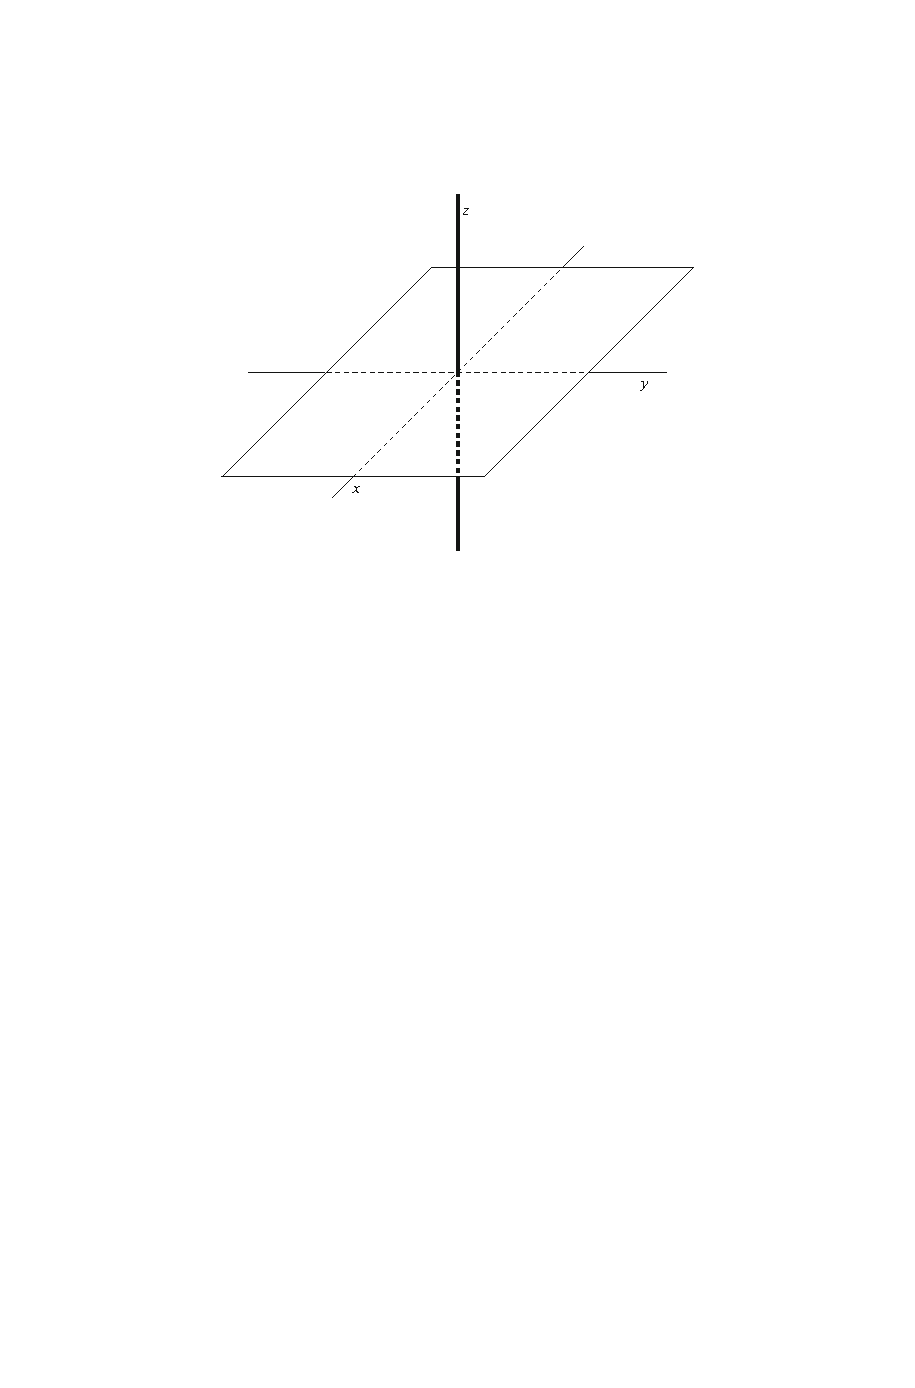
\includegraphics[width=0.4\linewidth]{Images/variety_dim.pdf}
    \caption{$\V(xz,yz)$ - a union of a line and a plane. From \cite{book:coxlittleoshea}}
    \label{fig:variety_dim}
\end{figure}
\begin{note}
    The ``dimension'' of a variety is not exactly as the dimension of vector space. See \ref{fig:variety_dim}, $\V(xz,yz)=\V(z)\cup\V(xy)$ as $xz=yz=0$ implies $z=0$ ($x-y$ plane) or $x=y=0$ ($z-$axis). The variety is a union of line and a plane, two different dimensional objects from linear algebra. Hence, the term needs to be defined appropriately first for an affine variety.
\end{note}
\section{Ideals}
\begin{defn}[Ideal]
    A subset $I\subseteq \F[x_1, x_2, \ldots, x_n]$ which satisfies the below properties is called an Ideal.
    \begin{itemize}
        \item $0 \in I$
        \item $f(x),g(x) \in I \Rightarrow f(x)+g(x)\in I, \forall x \in \F^n$
        \item $f(x) \in I \Rightarrow h(x)f(x)\in I, \forall h(x)\in \F[x_1, x_2, \ldots, x_n] \text{ and }\forall x \in \F^n$
    \end{itemize}
    As $I$ is subset, its operations are same as defined over $\F[x_1, x_2, \ldots, x_n]$.
\end{defn}
\begin{lem}
    For $f_1,f_2,\ldots,f_s\in\F[x_1, x_2, \ldots, x_n]$,  $\langle f_1,f_2,\ldots,f_s\rangle$ is the \emph{ideal generated} by $f_1,f_2,\ldots,f_s$. Also, $f_1,f_2,\ldots,f_s$ is a \emph{generating set} of $\langle f_1,f_2,\ldots,f_s\rangle$.
    \begin{equation}{\label{eq:ideallc}}
        I = \langle f_1,f_2,\ldots,f_s\rangle = \left\{\sum_{i=1}^{s}h_{i}\cdot f_{i}|h_i \in \F[x_1, x_2, \ldots, x_n]\right\}
    \end{equation}
    It is trivial to show that $\langle f_1,f_2,\ldots,f_s\rangle$ is indeed an ideal, use the representation \ref{eq:ideallc} and verify the three properties.
\end{lem}
Notice, how the definition of an ideal seems similar to a vector space, and \ref{eq:ideallc} looks similar to a linear combination. While multiplying, all polynomials are considered as ``scalars'' of the system. 
\begin{defn}[Finitely Generated Ideal]
    An ideal $I$ is finitely generated if
    \begin{equation}
        \exists f_1,f_2,\ldots,f_s \in \F[x_1, x_2, \ldots, x_n] \text{ such that }I=\langle f_1,f_2,\ldots,f_s\rangle
    \end{equation}
\end{defn}
\begin{defn}[Principle Ideal]
    An ideal $I$ generated by single element is a principle ideal.
\end{defn}
% $I=\langle f\rangle, f\in\F[x]$
\begin{defn}[Principle Ideal Domain (PID)]
    If every ideal in a domain is a principle ideal then the domain is called principle ideal domain.
\end{defn}
\begin{defn}[Ideal of an affine variety]
    The set $\I(V)$ is the ideal of an affine variety.
    \begin{equation}
        \I(V) =\{f\in\F[x_1, x_2, \ldots, x_n] \ |\ f(a_1, a_2, \ldots, a_n)=0, \forall a\in V\}
    \end{equation}
    It is trivial to show that $\I(V)$ is indeed an ideal, as for any $a\in V$:
    \begin{itemize}
        \item $0 \in \I(V)$ as $0(a) = 0, \forall a \in V$
        \item $f,g \in \I(V) \Rightarrow f(a) = g(a) = 0 \Rightarrow f(a)+g(a)=0 \Rightarrow f+g \in \I(V)$
        \item $f \in \I(V) \Rightarrow f(a) = 0 \Rightarrow h(a)f(a)=0 \Rightarrow hf \in \I(V)$
    \end{itemize}
\end{defn}
\begin{lem}
    For $f_1,f_2,\ldots,f_s\in \F[x_1, x_2, \ldots, x_n]$, $\langle f_1,f_2,\ldots,f_s\rangle\subseteq\I(V(f_1,f_2,\ldots,f_s))$
\end{lem}
\vspace{-1em}
\begin{proof}
    Take $f\in\langle f_1,f_2,\ldots,f_s\rangle\Rightarrow \exists h_i\in\F[x_1, x_2, \ldots, x_n]$ such that $f =\sum_{i=1}^{s}h_{i}\cdot f_{i}$\\
    Now, consider $a\in \V(f_1,f_2,\ldots,f_{s})\Rightarrow f_i(a)=0 \Rightarrow f(a)=0 \Rightarrow \I(V)$.
\end{proof}
\begin{note}
    The above containment need can be strict.\\
    Consider $f = x^2$,
    $I=\langle f\rangle=h\cdot f$,  $\forall h \in \F[x] \Rightarrow I$ contains polynomials of total degree $\geq 2$.\\
    But $V(f) = V(x^2)\Rightarrow V = \{0\} \Rightarrow g=x \in \I(V) \Rightarrow \I(V)$ contains polynomials of total degree 1.
    % The above containment need can be strict. Consider $f_i = x_i^2$,\\
    % $I=\langle f_1,f_2,\ldots,f_s\rangle=\sum_{i=1}^{s}h_{i}\cdot f_{i}$,  $h_i \in \F[x_1, x_2, \ldots, x_n] \Rightarrow I$ contains polynomials of total degree $\geq 2$.\\
    % But $\I(V)\Rightarrow x_i = 0 \Rightarrow g_i=x_i \in \I(V) \Rightarrow \I(V)$ contains polynomials of total degree 1.    
\end{note}
Similar to affine varieties, we can ask some interesting questions about ideals
\begin{description}
    \item[Ideal Description] Does every ideal $I\subseteq\F[x_1, x_2, \ldots, x_n]$ has a finite generating set.
    \item[Ideal Membership] If $I=\langle f_1,f_2,\ldots,f_s\rangle$, is there a way to determine if $f\in I$ .
    \item[Nullstellensatz] Is there an exact relation between $\langle f_1,f_2,\ldots,f_s\rangle$ and $\I(V(f_1,f_2,\ldots,f_s))$
\end{description}
Again, surprisingly, we can answer all these questions. See \ref{sec:gbintro}.
\section{Polynomials: Algorithms}
\begin{prop}[Divison Algorithm (Univariate Polynomials)]
    For every $f\in\F[x]$ and non-zero $g\in\F[x]$, $\exists! q,r\in\F[x]$ such that $f=qg+r$, where either $r=0$ or $\op{deg}(r)<\op{deg}(g)$.
\end{prop}
\vspace{-1em}
\begin{proof}
    Proof by construction, we ``divide'' $f$ by $g$ to get $q,r$.\\
    One thing to note is that, for non-zero $f,g$
    \begin{equation}
        \op{LT}(f) \text{ divides } \op{LT}(g) \Leftrightarrow \op{deg}(f) \leq \op{deg}(g)
    \end{equation}
    \begin{center}
        % \vspace{-1em}
        \begin{algorithm}
        \caption{Polynomial Division (Single Variable)}\label{alg:polynomialdivisionsingle}
        \begin{algorithmic}
        \Require $f,g$ where $f,g \in\F[x], g!=0$
        \Ensure $q,r$
        \State $q \gets 0$
        \State $r \gets f$
        \While{$r \neq 0$ and $\op{LT}(g)|\op{LT}(r)$  ($a|b$ is $a$ divides $b$) }
        % \If{$N$ is even}
        \State $q \gets q+\dfrac{\op{LT}(r)}{\op{LT}(g)}$
        \State $r \gets r-\dfrac{\op{LT}(r)}{\op{LT}(g)}g$ %\Comment{This is a comment}
        % \ElsIf{$N$ is odd}
        % \EndIf
        \EndWhile \\ 
        \Return $q,r$
        \end{algorithmic}
        \end{algorithm}
        % \vspace{-1em}
    \end{center}
    Note that, $f=qg+r$ always holds. It holds iniatilly and then,
    \begin{equation}
        f=qg+r \Leftrightarrow
        f=\left(q+\dfrac{\op{LT}(r)}{\op{LT}(g)}\right)g+\left(r-\dfrac{\op{LT}(r)}{\op{LT}(g)}g\right)
    \end{equation}
    The algorithm terminates because, $\op{deg}(r)$ drops at each iteration or $r$ becomes 0.\\
    Uniqueness follows from contradiction argument.
\end{proof}
\begin{note}
    If $r=0$ we say that $g$ \textbf{divides} $f$
\end{note}
\begin{theorem}[Divison Algorithm (Multivariate Polynomials)]
    For any $f\in\F[x_1, x_2, \ldots, x_n],\\ F=(f_1,f_2,\ldots,f_s)$  where $f_i \in\F[x_1, x_2, \ldots, x_n]$ on a monomial order, \\$\exists q_i, r\in\F[x_1, x_2, \ldots, x_n]$ where either $r=0$ or $r=\displaystyle\sum_{\alpha}a_\alpha\cdot x^\alpha, \op{LT}{f_i} \nmid x^\alpha, \forall i, \alpha$.\\
    Moreover, $q_i \cdot f_i\neq 0 \Rightarrow \op{multideg}(f)\geq\op{multideg}(q_i\cdot f_i)$
\end{theorem}
\begin{proof}
    Proof by construction, we divide $f$ by $f_i$ to get $q_i$, until we can't divide further (Division Step), then the leading terms move to remainder until one of them divides $f_{i+1}$ (Remainder Step). Now, divide by $f_{i+1}$ and repeat the steps till the end.
    \begin{center}
        % \vspace{-1em}
        \begin{algorithm}
        \caption{Polynomial Division (Multiple Variable)}\label{alg:polynomialdivisionmultiple}
        \begin{algorithmic} 
        \Require $F =(f_1,f_2,\ldots,f_s)$ and $f$ where $f,f_i\in\F[x_1, x_2, \ldots, x_n]$
        \Ensure $q_1,q_2,\ldots,q_s,r$
        \State $q_i \gets 0, \forall i$
        \State $r \gets 0$
        \State $p \gets f$
        \While{$p\neq0$}
            
            \State $i \gets 1$
            \State $\text{division} \gets \text{false}$
            \While{$i\leq s$ and $\text{division} = \text{false}$}
                \If{$\op{LT}(f_i)|\op{LT}(p)$}
                    \State $q_i \gets q_i+\dfrac{\op{LT}(p)}{\op{LT}(f_i)}$
                    \State $p \gets p-\dfrac{\op{LT}(p)}{\op{LT}(f_i)}f_i$
                    \State $\text{division} \gets \text{true}$
                \Else
                    \State $i \gets i+1$
                \EndIf
            \EndWhile
            \If{$\text{division} = \text{false}$}
                \State $r \gets r-\op{LT}(p)$
                \State $p \gets p-\op{LT}(p)$
            \EndIf
        \EndWhile \\
        \Return $q_1,q_2,\ldots,q_s,r$
        \end{algorithmic}
        \end{algorithm}
        % \vspace{-1em}
    \end{center}
    Proof is similar to \ref{alg:polynomialdivisionsingle} but lengthier.
    Here, $f=\displaystyle\sum_{i}q_i\cdot f_i+p+r$ always holds. It holds initially and then during division step,
    \begin{equation}
        q_i\cdot f_i+p \Leftrightarrow
        \left(q_i+\dfrac{\op{LT}(p)}{\op{LT}(f_i)}\right)f_i+\left(p-\dfrac{\op{LT}(p)}{\op{LT}(f_i)}f_i\right)
    \end{equation}
    and during the remainder step,
    \begin{equation}
        p+r \Leftrightarrow
        (p-\op{LT}(p))+(r+\op{LT}(p))
    \end{equation}
\end{proof}
\begin{note}
    In \ref{alg:polynomialdivisionmultiple}, the remainder and quotients are not uniquely determined, they may change with permutation of $F$. Applying the division algorithm on $f=xy^2-x$ over $F=(f_1,f_2)=(y^2-1, xy^2-x)$ gives $(q_1,q_2,r)=(x,0,0)\Rightarrow f\in \langle f_1,f_2\rangle$ whereas, over $F=(f_2,f_1)$ gives $(q_1,q_2,r)=(y,0,-x+y)$.\
\end{note}
\clearpage
\part{\Grob Bases: Introduction}
\section{Motivation: The Ideal Membership Problem}
Recall the Ideal Membership Problem. If $I=\langle f_1,f_2,\ldots,f_s\rangle$, is there a way to determine if $f\in I$?\\
We first look at the univariate case,
\begin{prop}{\label{eq:univariatepid}}
    For every ideal $I\subseteq\F[x]$, $\exists! f \in\F[x]$ such that $I=\langle f\rangle$. Also, this $f$ either is zero polynomial (iff $I=\{0\}$) or it is \emph{monic} $(i.e., \op{LC}(f)=1)$.\\This means that every ideal in $\F[x]$ is a principle ideal and $\F[x]$ is a principle ideal domain.
\end{prop}
\begin{proof}
We consider the cases,
    \begin{itemize}
        \item $I=\{0\}\Rightarrow I = \langle 0\rangle \Rightarrow f= 0$ and $\langle f\rangle=\langle 0\rangle=\{0\}$.
        \item $I\supset\{0\}$, we claim the monic polynomial of minimum degree in the ideal is such an $f$.
        \begin{itemize}
            \item $f\in I\Rightarrow \langle f\rangle\subseteq I$, since $I$ is an ideal. %Hence, $\langle f\rangle\subseteq I$
            \item For any $g\in I$, we can divide it by $f$ using \ref{alg:polynomialdivisionsingle} to get $g=qf+r$. As $g, f \in I\Rightarrow r \in I$. Now, $r$ is either 0 or $\op{deg}(r)<\op{deg}(f)$. Since the latter is not possible, $r=0$ which implies $g\in \langle f\rangle$. Hence $I\subseteq \langle f\rangle$.
        \end{itemize}
    \end{itemize}
    For uniqueness, $\langle f\rangle=\langle \tilde{f}\rangle \Rightarrow f = c\tilde{f}, \text{ where } c\in\F\setminus\{0\}\Rightarrow c = 1$ (as both $f,\tilde{f}$ are monic).
\end{proof}
This essentially solves the Ideal Membership Problem for ideals $\in\F[x]$.\\
A way to compute that $f$ is by calculating the \emph{GCD} of its generating set.
\begin{defn}[Greatest Common Divisor (GCD)]
    $g\in\F[x]$ is a greatest common divisor of $f_1,f_2,\ldots,f_s \in \F[x]$ if it satisfies the below properties,
    \begin{itemize}
        \item $g$ divides $f_1,f_2,\ldots,f_s$.
        \item $p$ divides $f_1,f_2,\ldots,f_s\Rightarrow p$ divides $g$
    \end{itemize}
    $g$ if exists is unique up to a multiplication by $c\in\F\setminus\{0\}$. As any gcd $g,\tilde{g}$ divides each other. We denote this gcd by $\op{gcd}(f_1,f_2,\ldots,f_s)$.
\end{defn}
\begin{prop}{\label{eq:gcdgenerator}}
    \begin{equation}
        I = \langle\op{gcd}(f_1,f_2,\ldots,f_s)\rangle=\langle f_1,f_2,\ldots,f_s\rangle
    \end{equation}
\end{prop}
\begin{proof}
    By \ref{eq:univariatepid}, $\exists f\in\langle f_1,f_2,\ldots,f_s\rangle$ such that $\langle f\rangle = \langle f_1,f_2,\ldots,f_s\rangle$. Now, $f=\op{gcd}(f_1,f_2,\ldots,f_s)$.
    \begin{itemize}
        \item Any $f$ divides $f_i$ as $f_i\in \langle f\rangle\Rightarrow f_i = h_i\cdot f$.
        \item Any $p$ divides $f_i\Rightarrow f_i = A_i\cdot p\Rightarrow f = \sum_{i}B_i \cdot f_i = \left(\displaystyle\sum_{i}A_i\cdot B_i \cdot\right) p \Rightarrow f$ divides $p$.
    \end{itemize}
    % \begin{itemize}
        % \item Since, $\op{gcd}(f_1,f_2,\ldots,f_s)$ divides $f_i$ for each $i$. It implies $f_i=A_i\cdot\op{gcd}(f_1,f_2,\ldots,f_s)\Rightarrow$ Any $f\in\langle f_1,f_2,\ldots,f_s\rangle\Rightarrow f = \sum_{i}h_i\cdot f_i\Rightarrow f = (\sum_{i}h_i\cdot A_i) g \Rightarrow f\in\langle\op{gcd}(f_1,f_2,\ldots,f_s)\rangle$. Hence, $\langle f_1,f_2,\ldots,f_s\rangle\subseteq \langle\op{gcd}(f_1,f_2,\ldots,f_s)\rangle$.
        % \item Since, $f\in\langle f_1,f_2,\ldots,f_s\rangle\Rightarrow  \op{gcd}(f_1,f_2,\ldots,f_s)\in\langle f_1,f_2,\ldots,f_s\rangle$. Hence $\langle\op{gcd}(f_1,f_2,\ldots,f_s)\rangle\subseteq\langle f_1,f_2,\ldots,f_s\rangle$.
    % \end{itemize}
\end{proof}
This GCD can be computed by applying Euclid's Algorithm successively to pairs of $f_1,f_2,\ldots,f_s$.
\begin{prop}[Euclid's Algorithm]{\label{algo:euclidgcd}}
    Euclid's Algorithm is used to compute $\op{gcd(f_1,f_2)}$ where $f_1,f_2 \in\F[x], f_2\neq0$.
    \begin{center}
        \begin{algorithm}
        \caption{Euclid's Algorithm}\label{alg:euclidgcd}
        \begin{algorithmic}
        \Require $f_1,f_2$ where $f_1,f_2 \in\F[x], f_2\neq0$
        \Ensure $g=\op{gcd}(f,g)$
        \State $g \gets f_1$
        \State $h \gets f_2$
        \While{$h \neq 0$}
        % \If{$N$ is even}
        \State $g,h \gets h, r \text{ where $r$ is the remainder of $g$ when divided by $h$ }(g=qh+r)$
        % \ElsIf{$N$ is odd}
        % \EndIf
        \EndWhile \\ 
        \Return $g$
        \end{algorithmic}
        \end{algorithm}
    \end{center}
    The algorithm terminates because, $\op{deg}(r)$ drops at each iteration or $r$ becomes $0$.
\end{prop}
\begin{theorem}[Ideal Membership Problem (Univariate Polynomial Ideals)]
For an ideal $I=\langle f_1,f_2,\ldots,f_s\rangle\subseteq\F[x]$, and $f,f_i\in\F[x]$,
    \begin{equation}
        f\in I\Leftrightarrow \op{gcd}(f_1,f_2,\ldots,f_s) \text{ divides } f.
    \end{equation}
\end{theorem}
\begin{proof}
    Trivial from \ref{eq:gcdgenerator}.
\end{proof}
Now, we move to ideals in domain of multivariate polynomials.

As seen at the end of \ref{alg:polynomialdivisionmultiple}, for a arbitrary generating set. The remainder when $f$ is divided by $F= (f_1,f_2,\ldots,f_s)$ need not be zero for all orderings of $F$. In worst case, we may need to check all permutations of $F$ until we get zero remainder. This can be shown to be \emph{worse than exponential complexity}. Hence, for a generating set, it is desirable that the remainder is 0 when divided by all possible orderings of $F$ iff $F$ divides $f$. In fact, such a generating set does exist for each ideal in $\F[x_1, x_2, \ldots, x_n]$. This set is the \textbf{\Grob Basis} of the ideal.

Before we jump onto it, let us understand Monomial Ideals.% as our understanding monomials gives better understanding of polynomials.
\subsection{Monomial Ideals}
\begin{defn}[Monomial Ideals]
    An ideal $I\subseteq \F[x_1, x_2, \ldots, x_n]$ is a monomial ideal if $\exists A\subseteq \Z^n_{\geq0}$ such that
    \begin{equation}
        I = \langle x^\alpha | \alpha\in A\rangle
    \end{equation}
    Intuitively, the ideal is generated by a set of monomials (possibly infinite).
    \end{defn}
\begin{lem}{\label{eq:everytermlies}}
    Given a monomial ideal $I$ and a $f\in\F[x_1, x_2, \ldots, x_n]$, $f\in I$ iff every term of $f$ lies in $I$.
\end{lem}
\begin{proof}
    The if direction is trivial since any $f$ is a linear combination of monomials.\\
    For the only if direction, consider the contrapositive, i.e., $\exists a_{\tilde{\alpha}} \cdot x^{\tilde{\alpha}}\notin I\Rightarrow f\notin I$.\\
    $a_{\tilde{\alpha}} \cdot x^{\tilde{\alpha}}\notin I\Rightarrow \forall \alpha \in A, x^\alpha$ doesn't divide $x^{\tilde{\alpha}}$. Hence, when we divide $f$ by the monomials of $I$, the remainder will always contain $x^{\tilde{\alpha}}$ or its multiple $\Rightarrow f\notin I$.
\end{proof}
\begin{theorem}[Dickson's Lemma]{\label{eq:dicksonlemma}}
    Every monomial ideal $I = \langle x^\alpha | \alpha\in A\rangle$ has a finite basis\footnote{we also call a generating set a basis. This is unlike the definitions from vector spaces.}, i.e., $\exists \alpha(1), \alpha(2), \ldots, \alpha(s)\in A$ such that $I = \langle x^{\alpha(1)}, x^{\alpha(2)}, \ldots, x^{\alpha(s)}\rangle$.
\end{theorem}
\begin{proof}
    The idea is to use induction on the number of variables. Base case $(n=1)$ follows from \ref{eq:univariatepid}. In inductive case, consider monomials in $\F[x_1, x_2, \ldots, x_{n-1}, y]$. They can be written as $x^\alpha y^m, \alpha\in \Z^{n-1}_{\geq0}$. Now, take $J$ as the ideal in $\F[x_1, x_2, \ldots, x_{n-1}]$ generated by $x^\alpha$ where $x^\alpha y^m\in I$. Use the inductive hypothesis to represent this $J$ with a finite generating set such that $J=\langle x^{\alpha(1)}, x^{\alpha(2)}, \ldots, x^{\alpha(s)}\rangle$. Now create, $m$ ideals $J_l\in\F[x_1, x_2, \ldots, x_{n-1}]$ where $0\leq l\leq m-1$ such that it is generated by monomials $x^\beta y^l\in I$. Again, by inductive hypothesis, $J_l$ has finite generating set. Now, $J\cup \bigcup_{l=0}^{m-1}J_l$ is a finite generating set of given monomial ideal.
\end{proof}
\begin{defn}[Minimal Basis]
    A monomial ideal $I=\langle x^{\alpha(1)}, x^{\alpha(2)}, \ldots, x^{\alpha(s)}\rangle$ has a minimal basis if $\forall i,j\ (i\neq j),\ x^{\alpha(i)}$ doesn't divide $x^{\alpha(j)}$. Also, this basis is unique.
\end{defn}
\begin{proof}
    Repeatedly remove the monomials which have divisors until it not possible. Uniqueness follows from contradiction arguments as monomials from two minimal basis will divide each other.
\end{proof}
\begin{theorem}[Ideal Membership Problem (Monomial Ideals)]
For a monomial ideal $I=\langle x^{\alpha(1)}, x^{\alpha(2)}, \ldots, x^{\alpha(s)}\rangle$ and a $f\in\F[x_1, x_2, \ldots, x_n]$ such that $f=\displaystyle\sum_{\alpha}a_\alpha \cdot x^\alpha$,
\vspace{-1em}
    \begin{equation}
        f\in I\Leftrightarrow \forall \alpha \exists i \text{ such that } x^{\alpha(i)} \text{ divides } x^\alpha.
    \end{equation}
\end{theorem}
\begin{proof}
    Application of \ref{eq:everytermlies} and \ref{eq:dicksonlemma}.
\end{proof}
\section{\Grob Bases}{\label{sec:gbintro}}
\begin{defn}
    For a non-zero ideal $I\subseteq\F[x_1, x_2, \ldots, x_n]\setminus$ and a monomial ordering on $\F[x_1, x_2, \ldots, x_n]$, we denote the set of leading terms of non-zero elements of $I$ as
    \begin{equation}
        \op{LT}(I)=\{a_\alpha x^\alpha|\exists f\in I\setminus\{0\} \text{ such that } \op{LT}(f)=a_\alpha x^\alpha\}
    \end{equation}
    % \begin{itemize}
    %     \item $\op{LT}(I)=\{a_\alpha x^\alpha|\exists f\in I\setminus\{0\} \text{ such that } \op{LT}(f)=a_\alpha x^\alpha\}$
    %     \item $\langle \op{LT}(I)\rangle$ is the ideal generated by $\op{LT}(I)$
    % \end{itemize}
    The motivation for this definition is then, $\langle \op{LT}(I)\rangle$ is a monomial ideal. So by \ref{eq:dicksonlemma}, it has a finite basis.
\end{defn}
\begin{theorem}[Hilbert Basis Theorem]{\label{eq:hilbertbasistheorem}}
    Every ideal $I\subseteq \F[x_1, x_2, \ldots, x_n]$ has a finite basis.
\end{theorem}
Note, the Hilbert Basis Theorem solves the \textbf{Ideal Description} problem.
\begin{proof}
    For $I=\{0\}$, we have $I=\langle 0\rangle$. For other $I$, by \ref{eq:dicksonlemma} $\exists g_1, g_2, \ldots, g_t\in I$ such that $\langle \op{LT}(I)\rangle=\langle \op{LT}(g_1), \op{LT}(g_2), \ldots, \op{LT}(g_t)\rangle$. Now, we can show that $I=\langle g_1, g_2, \ldots, g_t\rangle$, by dividing $f\in$ with $G = (g_1, g_2, \ldots, g_t)$ and proving that the remainder is zero.
\end{proof}
\begin{theorem}[Ascending Chain Condition]{\label{eq:ascendingchaincondition}}
    $I_i\in\F[x_1, x_2, \ldots, x_n], \forall i\in\Zp$ such that $I_i\subseteq I_{i+1}\Rightarrow \exists N\in\Zp$ such that $I_{N}=I_{N+1}$.
    Intuitively, it states that the sequence of ideals where previous ideals are contained within current ideal stabilizes.
\end{theorem}
\begin{proof}
    Consider $I=\bigcup_{i=1}^\infty I_i$, clearly, $I$ is an ideal. Now, by \ref{eq:hilbertbasistheorem}, it has a finite generating set where each of its generator $f_i$ is contained in some $I_{j_i}$. This implies due to ascending chain, all generators are contained in $I_N$ where $N=\max_{i}j_i\Rightarrow$ generators of $I_k$ where $k\geq N$ are same. So, $I_N=I_{N+1}$
\end{proof}
\begin{defn}[Affine Variety of an Ideal]
    For an ideal $I\subseteq\F[x_1, x_2, \ldots, x_n]$ such that $I=\langle f_1,f_2,\ldots,f_s\rangle$, the affine variety of an Ideal is defined as below,
    \begin{equation}
        \V(I) = \V(f_1,f_2,\ldots,f_s) = \{(a_1, a_2, \ldots, a_n) \in \F^n \ |\ f(a_1, a_2, \ldots, a_n)=f(a)=0 \ \forall f\in I \}
    \end{equation}
\end{defn}
\begin{defn}[\Grob Basis]
    For a fixed monomial ordering on $\F[x_1, x_2, \ldots, x_n]$ and \\$G = \{g_1, g_2, \ldots, g_t\}$, $G$ is called a \Grob basis of a non-zero ideal $ I  \subseteq\F[x_1, x_2, \ldots, x_n]$ if
    \begin{equation}
        \langle \op{LT}(I)\rangle = \langle \op{LT}(g_1), \op{LT}(g_2), \ldots, \op{LT}(g_t)\rangle
    \end{equation}
    The \Grob basis of $I=\{0\}$ is defined as $\varnothing$.
\end{defn}
\begin{prop}[Property of \Grob Bases]
    For a \Grob basis $G = \{g_1, g_2, \ldots, g_t\}$ for an ideal $I\subseteq\F[x_1, x_2, \ldots, x_n]$ and a given $f\in\F[x_1, x_2, \ldots, x_n]$, $\exists!r\in\F[x_1, x_2, \ldots, x_n]$ such that no term of $r$ is divisible by $\op{LT}(g_i)$ for any $i$.

    The uniqueness of remainder is the reason the ordered tuple we divide with is a set.
\end{prop}
\begin{note}
    Only remainder is guarenteed to be unique, the quotients need not be unique.
\end{note}
\begin{theorem}[Ideal Membership Problem (Multivariate Polynomial Ideals)]
    For a \Grob basis $G = \{g_1, g_2, \ldots, g_t\}$ for an ideal $I\subseteq\F[x_1, x_2, \ldots, x_n]$,
    \begin{equation}
         f\in I\Leftrightarrow \text{ remainder on division of } f \text{ by } G \text{ is zero}.
    \end{equation}
\end{theorem}
\subsection{Computation of \Grob Basis}
\begin{defn}Here are some additional notations that will be helpful.
    \begin{itemize}
        \item $\overline{f}^F$ is the remainder on division of $f$ by $F=(f_1,f_2,\ldots,f_s)$.
        \item $x^\gamma=\op{lcm}(\op{LM}(f),\op{LM}(g))$, i.e., it is the least common multiple of $\op{LM}(f),\op{LM}(g)$\\ with $\gamma_i=\max(\alpha_i,\beta_i)$ where $\op{multideg}(f)=\alpha, \op{multideg}(g)=\beta$.
        \item $S(f,g)=\left(\dfrac{x^\gamma}{\op{LT}(f)}\cdot f-\dfrac{x^\gamma}{\op{LT}(g)}\cdot g\right)$ is the S-polynomial of $f,g$.
    \end{itemize}
\end{defn}
\begin{theorem}[Buchberger's Criterion]{\label{eq:buchbergercriterion}}
    A basis $G = \{g_1, g_2, \ldots, g_t\}$ is a \Grob basis of $I\subseteq\F[x_1, x_2, \ldots, x_n]$ iff $\overline{S(g_i,g_j)}^G=0, \forall i,j\ (i\neq j)$
\end{theorem}
\begin{theorem}[Buchberger's Algorithm]{\label{algo:buchberger}}
    For a non-zero ideal $I=\langle f_1,f_2,\ldots,f_s\rangle$, \Grob basis for $I$ is constructed as follows:\\
    Given a basis, we can extend the basis to a \Grob basis by repeatedly adding the non-zero remainders of S-polynomials between pairs of basis to the basis until \ref{eq:buchbergercriterion} is satisfied.
\end{theorem}
\begin{center}
    % \vspace{-1em}
    \begin{algorithm}
    \caption{Buchberger's Algorithm}\label{alg:polynomialdivisionsingle}
    \begin{algorithmic}
    \Require $F=(f_1,f_2,\ldots,f_s)$ where $f_i$'s are non-zero
    \Ensure $G=(g_1, g_2, \ldots, g_t)$ where $G$ is a \Grob Basis for $I$
    \State $G \gets F$
    \Repeat
    \State $G^\prime \gets G$
    \For {all pairs $\{p,q\}$ where $p,q \in G^\prime, p\neq q$}
    \State $r\gets \overline{S(p,q)}^{G^\prime}$
    \If {$r\neq0$}
    \State $G\gets G\cup\{r\}$
    \EndIf
    \EndFor
    \Until {$G=G^\prime$}\\
    \Return $G$
    \end{algorithmic}
    \end{algorithm}
    % \vspace{-1em}
\end{center}
\begin{proof}
    In the beginning, $G\in I$, let each iterate of $G$ be called $G^{(i)}$. Now, if $G^{(i)}\in I$then whenever a remainder $r=\overline{S(g_i,g_j)}^{G^{i}}$ is added to $G^{(i)}$ then $G^{(i+1)}\in I$ as $r\in I$. As $F\subseteq G and \langle F\rangle=I\Rightarrow \langle G\rangle=I$. So, the algorithm if terminates gives a \Grob basis.\\
    Now, due to addition of $r$, $\langle \op{LT}(G^{(i)})\rangle\subseteq\langle \op{LT}(G^{(i+1)})\rangle$, so this sequence forms an ascending chain and thus, by \ref{eq:ascendingchaincondition} it converges. Hence, the algorithm terminates.
\end{proof}
\begin{defn}[Reduced \Grob Basis]
    A reduced \Grob basis $G = \{g_1, g_2, \ldots, g_t\}$ of an ideal $I\subseteq\F[x_1, x_2, \ldots, x_n]$ is such that $\forall i, \op{LC}(g_i)=1$ and no monomial of $g_i$ belongs to $\langle \op{LT}(G\setminus\{g_i\})\rangle$.\\
    Also, a reduced \Grob basis is unique for an ideal subject to monomial ordering.
\end{defn}
Such, a \Grob basis can be constructed by repeatedly removing $g_i$ where $\op{LT}(g_i)\in\langle \op{LT}(G\setminus\{g_i\})$. These new sets are also a \Grob basis.

Note, the process of computing \Grob basis is very expensive but once computed, we can solve plethora of applications as we will see in next parts.
\clearpage
\part{Algebra and Geometry: Interconnection}
\section{Nullstellensatz}{\label{sec:nullstellensatz}}
The following results are taken from \cite{book:coxlittleoshea}.
\begin{theorem}[The Weak Nullstellensatz]
    For an algebraically closed field $\F$ and if $I\subseteq\F[x_1, x_2, \ldots, x_n]$ is an ideal satisfying $\V(I)=\varnothing$ then $I=\F[x_1, x_2, \ldots, x_n]$
    Intuitively, this means that every system of polynomials than generates an ideal strictly smaller than $\F[x_1, x_2, \ldots, x_n]$ has a zero in $\C^n$.
\end{theorem}
This theorem allows us to solve the \textbf{consistency} problem,
\begin{cor}[Consistency Problem]
    $V = \V(f_1,f_2,\ldots,f_s)=\varnothing \Leftrightarrow$ the reduced \Grob basis of $I=\langle f_1,f_2,\ldots,f_s\rangle$ is \{1\}
\end{cor}
\begin{theorem}[Hilbert's Nullstellensatz]
    For an algebraically closed field $\F$ and if $f, f_i\in\F[x_1, x_2, \ldots, x_n]$ then
    \begin{equation}
        f \in \I(\V(f_1,f_2,\ldots,f_s)) \Leftrightarrow \exists m\geq1 \text{ such that } f^m \in \langle f_1,f_2,\ldots,f_s\rangle
    \end{equation}
\end{theorem}
\begin{defn}[Radical Ideal]
    For a radical ideal $I$, $f^m\in I$ for some $m\geq1\Rightarrow f\in I$.
\end{defn}
\begin{defn}[Radical of Ideal]
    The radical of an ideal $I\in\F[x_1, x_2, \ldots, x_n]$ is denoted by $\sqrt{I}$ which is defined as
    \begin{equation}
        I \subseteq \sqrt{I}=\{f|f^m\in I \text{ for some $m\geq1$}\} 
    \end{equation}
    Also, $\sqrt{I}$ is a radical ideal.
\end{defn}
\begin{theorem}[The Strong Nullstellensatz]
    For an algebraically closed field $\F$ and if $I\subseteq\F[x_1, x_2, \ldots, x_n]$ is an ideal then
    \begin{equation}
        \I(\V(I))=\sqrt{I}
    \end{equation}
\end{theorem}
\begin{theorem}[The Ideal–Variety Correspondence]  
    For an arbitrary field, $\I,\V$ are inclusion reversing, i.e.,
    \begin{equation}
        \begin{aligned}
            I_1\subseteq I_2\Rightarrow \V(I_1)\supseteq \V(I_2)\\
            V_1\subseteq V_2\Rightarrow \I(V_1)\supseteq \I(V_2)
        \end{aligned}
    \end{equation}
\end{theorem}
\clearpage
\part{\Grob Bases: Applications}
\section{Elimination Theory}{\label{sec:eliminationtheory}}
Recall that the \Grob basis  generalizes the idea of gcd as seen from the Ideal Membership problem for  polynomial ideals in one variable.
Now, we will see that it \Grob basis also generalizes the notion of rref and the process of ``elimination'' of variables is crucial one. This was hinted back then during our solving of polynomial equations with total degree one which were systems of linear equations from linear algebra.

Now, the key to eliminating variables from systems of polynomial equations lies in two step
\begin{description}
    \item[Elimination Step] With which we can eliminate certain variables from the equation to get ``simpler'' equations to work with and find solutions.
    \item[Extension Step] Once we have solutions for ``simpler'' equations we can extend these to get solutions of original equations.
\end{description}
\begin{defn}[Elimination Ideal]
    For an ideal $I=\langle f_1,f_2,\ldots,f_s\rangle\subseteq\F[x_1, x_2, \ldots, x_n]$, the $l-$\textsuperscript{th} elimination ideal $I_l$ is the ideal in $\F[x_{l+1}, x_{l+2}, \ldots, x_n]$ defined by
    \begin{equation}
        I_l = I \cap \F[x_{l+1}, x_{l+2}, \ldots, x_n]
    \end{equation} 
    Intuitively,   $I_l$  consists of functions in $I$ which eliminate the variables $x_1, x_2, \ldots, x_l$. Hence, the \emph{elimination step} is to determine elements of $I_l$.
\end{defn}
\begin{theorem}[The Elimination Theorem]
    For an ideal $I=\subseteq\F[x_1, x_2, \ldots, x_n]$ and its \Grob basis $G$ with respect to lex order $(x_1>x_2>\cdots>x_n)$,
    \begin{equation}
        G_l = G \cap \F[x_{l+1}, x_{l+2}, \ldots, x_n]
    \end{equation}
    where $G_l$ is the \Grob basis of the $l-$\textsuperscript{th} elimination ideal.
\end{theorem}
\begin{proof}
    $G_l\subseteq I_l$ by definition. Now, for $f\in I_l\Rightarrow f\in I\Rightarrow \exists g\in G$ such that $\op{LT}(g)$ divides $\op{LT}(f)\Rightarrow \op{LT}(g)\in\F[x_{l+1}, x_{l+2}, \ldots, x_n]\Rightarrow g \in \F[x_{l+1}, x_{l+2}, \ldots, x_n] \text{ due to lex order $(x_1>x_2>\cdots>x_n)$ }\Rightarrow g \in G_l\Rightarrow I_l \subseteq \langle G_l\rangle$.
\end{proof}
\begin{theorem}[The Extension Theorem]
    For an ideal $I=\langle f_1,f_2,\ldots,f_s\rangle\subseteq\C[x_1, x_2, \ldots, x_n]$ if its first elimanation ideal is $I_1$. Then,
    \begin{equation}
        f_i = c_i(x_2,\ldots,x_n)x_1^{N_i} + \text{ terms in $x_1$ with degree $< N_i$}\ (N_i\geq0, c_i\in\C[x_2, \ldots, x_n]\setminus\{0\})
    \end{equation}
    If there exists a partial solution $(a_2, \ldots, a_n)\in \V(I_1)$ \\
    then $(a_2, \ldots, a_n)\notin \V(c_1, c_2, \ldots, c_s)\Rightarrow \exists a_1\in \C$ such that $(a_1, a_2, \ldots, a_n)\in \V(I)$.
\end{theorem} 
Notice, how the working field is now $\C$, an algebraically closed field.
\section{Implicitization Problem}
The problem is to find implicit polynomial equations that represent a variety $V\in\F^n$ using parametrised variables. 
\begin{equation}
    x_i= f_i(t_1,t_2,\ldots,t_m) \text{ (for all $i$)}
\end{equation}
\begin{theorem}[Polynomial Implicitization]
    For an infinite field $\F$, $F:\F^m:\F^n$ denotes the parametrization and an ideal
    \begin{equation}
         I=\langle x_1-f_1,x_2-f_2, \ldots, x_n-f_n\rangle\subseteq\F[t_1,t_2,\ldots,t_m, x_1, x_2, \ldots, x_n]
     \end{equation} and $I_m$ be its $m$\suth elimination ideal. Then $\V(I_m)$ is the smallest variety in $\F^n$ containing $F(\F^m)$.
\end{theorem}
Hence, we can compute \Grob basis with respect to lex order such that every $t_i$ is higher than $x_i$.
\begin{theorem}[Rational Implicitization]
    For an infinite field $\F$, $F:\F^m\setminus W:\F^n$ denotes the parametrization and an ideal
    \begin{equation}
        x_i= \dfrac{f_i(t_1,t_2,\ldots,t_m)}{g_i(t_1,t_2,\ldots,t_m)} \text{ (for all $i$)} \text{ \quad and\quad } g=g_1g_2\cdots g_n,W=\V(g)
    \end{equation}
    \begin{equation}
        I=\langle g_1x_1-f_1,g_2x_2-f_2, \ldots, g_nx_n-f_n, 1-gy\rangle\subseteq\F[y,t_1,t_2,\ldots,t_m, x_1, x_2, \ldots, x_n]
    \end{equation}
    $I_{m+1}$ be its $(m+1)$\suth elimination ideal. Then $\V(I_{1+m})$ is the smallest variety in $\F^n$ containing $F(\F^m\setminus W)$.
\end{theorem}
Hence, we can compute \Grob basis with respect to lex order such that $y$ and every $t_i$ is higher than $x_i$.

Now, let us look at concrete applications which uses Elimination Theory to solve for polynomial equations. The entire code for these are available \href{https://github.com/paramrathour/Groebner-Basis-Applications}{here}. I will also add programs for even more applications.
\section{System of Linear Equations}
The problem of our interest is 
\begin{equation}
    Ax=b \quad(A\in \F^{n\times n}, \text{ and } b,x\in\F^{n\times 1})
\end{equation}
To convert the problem into polynomial equations, we rewrite it as
\begin{equation}
    f_i(x_1, x_2, \ldots, x_n) = -b_i + a_{i,1}x^1 + a_{i,2}x^2 + \cdots + a_{i,n}x^n = -b_i + \sum_{j=1}^n a_{i,j}x^j = 0 (1\leq i,j\leq n)
\end{equation}
where $a_{i,j}$ is the entry in the $i$\suth row and $j$\suth column of $A$ and $b_i$ is the entry in the $i$\suth row of $B$.

Then, we construct an ideal $I=\langle f_1,f_2,\ldots,f_n\rangle$ and find its \Grob basis $G$.

If the system has no solution then $G=\{1\}$, else the polynomials of $G$ give exactly the row reduced echelon form of the augmented matrix $[A:b]$. To solve such a system, we use 
Back-Substitution. This is akin to applying extension theorem to the ideals $I_{l}$.

The SageMath program to symbolically compute \textbf{all solutions} is attached at the end and can also be found \href{https://github.com/paramrathour/Groebner-Basis-Applications/blob/main/System of Linear Equations Symbolic Solver.ipynb}{here}
% \includepdf[pages=-]{System of Linear Equations Symbolic Solver.pdf}
% \begin{minted}[frame=single]{python}
% def solve_linear_system(F, A, B, n): # inputs: Field F, SageMath matrices A, B and n
%     solution = []
%     P = PolynomialRing(F, n, names='x', order='lex')
%     x = P.gens()
%     X = matrix([[x[i]] for i in range(n)]); X
%     equations = A*X-B
%     I = Ideal([equations[i][0] for i in range(n)])
%     print("The Ideal Corresponding to the equations is I = ", I)
%     gb = I.groebner_basis()
%     print("Groebner Basis of I is ", gb)

%     rref = [list(gb[i].dict().items()) for i in range(len(gb))];
    
%     if len(rref) == 1 and sum(rref[0][0][0]) == 0 and rref[0][0][1] == 1:
%         print("No Solution!, Exiting")
%         return solution
    
%     is_pivot_variable =  [0 for i in range(n)] # get alll pivot variables
%     for li in rref:
%         is_pivot_variable[[i for i, x in enumerate(li[0][0]) if x][0]] = 1
        
%     answer = []  # computes B part of rref(A:B)
%     for i in range(n):
%         if is_pivot_variable[i] == 0:
%             answer.append(var('c'+str(i), domain = CC))
%         else:
%             answer.append(rref[i][-1][-1])
    
%     for i in range(n): # back-substitution
%         for j in rref[i]:
%             indices = [k for k, x in enumerate(j[0]) if x]
%             if len(indices) != 0:
%                 index = indices[0]
%                 if index != i and index < n:
%                     answer[i] = answer[i] + answer[index]*j[1]
                    
%     for i in range(n):
%         solution.append(answer[i])
%     return solution
% \end{minted}
\section{System of Polynomial Equations}
The problem is to solve, $f_i(x)=0$ where $f_i\in\F[x_1, x_2, \ldots, x_n]$
Similar to the first problem, we construct an ideal $I=\langle f_1,f_2,\ldots,f_n\rangle$ and find its \Grob basis $G$.

If the system has no solution then $G=\{1\}$, else the polynomials of $G$ are in eliminated form. To solve such a system, we use Back-Substitution. This is akin to applying extension theorem to the ideals $I_{l}$. In this case, we will have to solve polynomial equations in one variable, which may require numerical approximation techniques for higher degree. 

The SageMath program to symbolically compute \textbf{some solutions} is attached at the end and can also be found \href{https://github.com/paramrathour/Groebner-Basis-Applications/blob/main/System of Polynomial Equations Solver.ipynb}{here}.
\section{Sudoku}
The objective is to fill a $m\times m$ grid ($m=n^2$) with integers from $1$ to $m$ such that no row or column or block has a same number appear twice. Any such board, can be represented in the block matrix form with its each entry being a \emph{block} of dimension $n\times n$.\\
We model a sudoku using Boolean Polynomials by creating $m\cdot (m^2)=m^3$ variables. $m$ boolean variables for every element of the grid. Let these variables be denoted by $x_{i,j}$ where $0\leq i\leq m^2-1$ and $0\leq j \leq m-1$, where $i$ represents the element number and $j$ represents the value that element can take.\\
There are three kinds of polynomial equations to be created to denote the following conditions,
\begin{itemize}
    \item for every $i$, exactly one of $x_{i,j}$ must be 1. This is achieved using following,
    \begin{equation}
        \begin{aligned}
            \forall i, \sum_{j=0}^{m-1}\prod_{k\neq j} x_{i,k} &= 0 \text{ (for each $i$, $x_{i,j} = 0$ for atleast $m-1$\ $j$'s)}\\
            \forall i, \sum_{j=0}^{m-1} x_{i,j} &= 1 \text{ (for each $i$, not all $x_{i,j} = 0$) }
        \end{aligned}
    \end{equation}
    \item for $i_1,i_2$ such that they are in same row or column or block, they should not have the same number.
    \begin{equation}
        \sum_{j=0}^{m-1} x_{i_1,j}\cdot x_{i_2,j} = 0 \text{ (for all valid  $(i_1, i_2)$ pairs)}
    \end{equation}
    \item encode the given value, if $x_i$ is $k$ then $x_{i,j}=1$ iff $j==k-1$. (i.e., other $x_{i,j}=0$)
\end{itemize}
Now, create an ideal and add all the equations to it as polynomials and find its \Grob basis $G$.
\begin{itemize}
    \item If the system has no solution then $G=\{1\}$, else the polynomials of $G$ are in eliminated form.
    \item If $G$ contains $m^3$ polynomials then there is a unique solution since each of the $m^3$ variable will have it's own linear equation (as $x^2=x$ for binary numbers) which is $x=0$ or $x+1=0$.
    \item If $G$ contains less than $m^3$ polynomials but more than one then $x$'s can be both $0$ or $1$ and $x$ is either eliminated from the equation or it is uniquely dependent on other variables which are eliminated at a later stage  and the number of elements in $G$ would be less than $m^3$.
\end{itemize}

Hence, solving if a unqiue solution exists is trivial but if more than one solutions are possible then to solve such a system, we use Back-Substitution. This is akin to applying extension theorem to the ideals $I_{l}$.
The SageMath program to symbolically compute \textbf{all solutions} is attached at the end and can also be found \href{https://github.com/paramrathour/Groebner-Basis-Applications/blob/main/Sudoku Solver.ipynb}{here}. Note, even after having $1000+$ equations the solution is calculated within 2 minutes if unique.
\begin{note}
    Our approach was very similar to integer programming and in fact, it can be changed a bit (by changing the field) to apply for integer programs as well. 
\end{note}
\addcontentsline{toc}{section}{References}
\nocite{*}
% \bibliographystyle{plainurl}
% \bibliography{ref}
\printbibliography
% \addcontentsline{toc}{section}{Modified Plan of Action}
\end{document}